\section{Additional Trigger Cost Considerations}\label{sec:additional_trigger_cost}

This section contains additional material concerning cost evaluations. The
trigger challenges for 2017 operation are addressed in
Section~\ref{ssec:trigger_2017}.  Estimations of the \rnn{} impact in the full
menu using cost monitoring results is later considered
(Section~\ref{ssec:cpu_2017_estimations}). Finally, we bring insights from Run~2
P1 data with strategies to maximize the impact in CPU savings for future
operations (Section~\ref{ssec:menu_cpu}).

\subsection{Trigger Challenges for 2017 Operation}\label{ssec:trigger_2017}

\begin{figure}[b]
\centering
\includegraphics[width=.7\textwidth]{cpu_extrapolations}
\caption{\label{fig:cpu_extrapolations}
Exponential fits of the number of cores (non-horizontal dashed lines), where
40,000 CPUs are normalized to the full processing power available for all
computational tasks (including \hlt{} processing) performed in P1 during 2016, as
a function of the online pile-up estimator (\avgmu{}) when employing measurements
performed in the P1 on different runs and menu versions (configurations in top
left legend). A horizontal dotted red line represents the expected computing
power for 2017 (48,000 CPU nodes, see text). The P1 estimations for
the 2017 preliminary menus dedicated to high luminosity operation
($\text{1.7e34}$ and \SI[parse-numbers =
false]{2.0e34}{\per\square\cm\per\second}) are shown by stars at their expected
pile-up maxima with horizontal dashed lines emphasizing the result of the
estimation. Circular points show a linear extrapolation based on the standard
CPU cost estimation (EB) for preliminary menus dedicated for data-taking on
luminosities up to $\text{1.7e34}$, $\text{1.9e34}$ and \SI[parse-numbers =
false]{2.0e34}{\per\square\cm\per\second}~\cite{ATR-16227}. Extracted
from~\cite{Martin2017b}.}
\end{figure}

Although ATLAS regarded as acceptable pile-up conditions up to $\avgmu=60$
during the preparation for data-taking after 2017 Technical Stop 1 (TS1), a
major concern considered the CPU processing power. CPU measurements on actual
operation of 2016 menu foreseen a minimal requirement of \SI{50}{\%} above 2016
available processing resources under pile-up conditions expected after TS1
(Figure~\ref{fig:cpu_extrapolations}), while only \SI{20}{\%} additional power
was enrolled~\cite{Shaw2017}. To allow measurement of improvements in the menu,
standard procedure employed for CPU cost measurements were used, which also
pointed to the direction of an urgent need for optimization of the
\hlt~\cite{Martin2017a,Shaw2017,Martin2017b}.  The campaign allowed to recover
\SI{20}{\%} of the processing power~\cite{Shaw2017}. However, a harsh
development scenario arose due to precision limitations of the standard CPU
measurements to predict a realistic data-taking scenario. In order to reduce
uncertainties in the estimations, two runs before TS1 employed a preliminary
version of the high luminosity menus~\cite{Stelzer2017}. Although extrapolations
of the new configuration resulted in a much less stringent scenario
(Figure~\ref{fig:cpu_extrapolations}), the reason for their lower dependency
with respect to \avgmu was not clear~\cite{ATR-16463}. Even in such projections,
the menu dedicated for data-taking on luminosity up to
$\SI{2.0e34}{\per\square\cm\per\second}$ raised concern for its high expected
CPU demands~\cite{ATR-16463}.

In addition to the aforementioned scenario, complementary processing power
expected for 2017 was not provided~\cite{Love2017}. Hence, this further required
a cost-reduction campaign during TS1~\cite{Leonidopoulos2017}, where the \rnn
was defined to be the baseline algorithm for electron chains. These efforts
allowed stable operation for the targeted pile-up benchmark despite the
processing power being kept similar to the available in 2016.

Finally, a problem in the sector 16L2 of the LHC was identified in August 2017
which required an alternative filling scheme (\emph{8b4e}: eight bunches filled,
four empty) and resulted in higher pile-up conditions for the same instantaneous
luminosity when compared to the nominal LHC operation. The menu evaluated for
these pile-up conditions ($\avgmu=80$) would have impacted in the physics
programme, thus the leveling of the instantaneous luminosity at
\SI{1.56e34}{\per\square\cm\per\second}, culminating in $\avgmu=60$, was
requested to the LHC~\cite{ATL-DAQ-PUB-2018-002}. When all facts are put
together, the relevance of the improvements performed in terms of CPU
optimization becomes clear as, otherwise, the conditions for 2017 data-taking
would impose limitations for some physics analyses.


\FloatBarrier
\subsection{2017 Cost Monitoring Results}\label{ssec:cpu_2017_estimations}

Figure~\ref{fig:chain_cpu_comp_2016_2017}
summarizes the cost reprocessing results\footnote{Background efficiency
measurements in Appendix~\ref{ssec:2017_cost_background_eff}.} obtained during
the first half of 2017. For instance, the tracking algorithms demanded
\SI{28}{\milli\second\per\text{event}} (\SI{86}{\milli\second\per\text{event}})
for all electron triggers when the menu was run with (without) \rnn{} as the
baseline algorithm. A similar reduction can be seen for the \hltcalo{} and the
final \hlt{} selection steps. These are due to the better \rnn{} discrimination
at the \fastcalo{}, i.e.\@ resulting in an increase of the fake rate reduction
factor from \SI{3.64}{$\times$} to \SI{9.11}{$\times$} (central value) for the
configuration as similar as possible to the lowest-energy-threshold unprescaled
single electron trigger monitored in these data reprocessing.

Taking into account the raw measurements, a \SI{25}{\%}
reduction in CPU demand of the full electron and photon triggers (\egamma{}
slice) was estimated when adopting the \rnn{} algorithm. Later, these results
were found to be lacking adjustments to account for differences in processing
conditions (LCG sites, load during processing time etc.). The reduction factor
after applying the correction procedure is of \SI{8}{\%}, yet relevant
specially when considering that \rnn{} affected only electron trigger legs above
\SI{15}{\GeV}.

Finally, it is worth mentioning that although the 2016 menu was evaluated with a
distinct set of triggers (MC\_v6\_tightperf), the reported results are similar
to the equivalent physics menu~\cite{RyanComment_ATR-15989}. In 2016, a
likelihood selection based only on shower-shape variables was being employed. It
was removed for 2017 execution, and the menu was optimized to maximize caching
in triggers assessing the same RoI. The \rnn-based menu is applied on top of the
caching improvements.

\begin{figure}[ht]
\centering
\includegraphics[width=\textwidth]{chain_comp_2016_2017}%
\caption{%
\label{fig:chain_cpu_comp_2016_2017}%
\hlt CPU time (central value) per event of bunch-crossing evaluated on EB stream
of run 309640 with 2016 menu on top (AtlasP1-21.0.9, MC\_v6\_tightperf,
ATR-15453), 2017 menu without \rnn on middle (AtlasP1-20.0.11,
Physics\_v7\_tight, ATR-15954) and the final 2017 menu, with \rnn, on bottom
(AtlasP1-20.0.19, Physics\_v7\_tight, ATR-15956). The number of
variables, their representation type and selection method for each menu and step
are displayed in a dedicated box. Contributions to the CPU total time per event
are divided accordingly to the processing steps. All CPU time is shown in units
of ms per event. They are further separated in three categories: first line
refers to CPU demands of all electron triggers; some of the \fastelectron
algorithms can only be assessed by evaluating their full menu time, displayed in
the second line; and hypothesis testing for a typical electron trigger is in the
third line, given that their measurements are obtained separately for each
working point and energy threshold. Contributions shown with arrows in pure red
refers exclusively to computations of ID information. It is displayed the
reduction factor of executions in the next step, except for the last one, where
the reduction factor is computed in terms of executions with respect to the
number of accepted events, for the lowest \et{} \tight{} trigger allowing to
access these informations. In the right, the total CPU per event for both
electron and photon triggers in each menu (highlighted in red) and the \hlt
output rate for electron triggers only (grey).  See~\cite{ATR-15957} for more
information on these measurements.}
\end{figure}

\FloatBarrier
\subsection{Maximizing the Impact in CPU Resources}\label{ssec:menu_cpu}

Precise measurement of the CPU impact during operation is not a trivial
task due to the frequent changes in the menu configuration. Although it was not
possible to find data-taking conditions with and without the \rnn operation
similar enough to allow conclusive measurements, we assessed the standard cost
monitoring data\footnote{2015 runs are not included due to differences in the
cost monitoring data format.} for insights concerning the Run~3 developments.
These data are sampled for a few luminosity blocks\footnote{Usually a data-taking
period of about \SI{60}{\second}.}, usually with a single block with less
detailed measurements or three successive blocks with more detailed
measurements, where about \SI{10}{\%} of the first level events are monitored.

Figure~\ref{fig:run2_monitored_cpu_per_group} shows that the \egamma{} triggers
were usually the second most-demanding group during data taking, except for
after 2017 TS1, where they were the most-demanding. B-jet group demanded more CPU
time than \egamma{} up to 2017 TS1, while in 2018 the top-most demanding group
was b-physics.  Figure~\ref{fig:run2_monitored_cpu_per_mu} shows that this
behavior roughly did not change according to menu configurations or runs within
each period. When taking into account the time per signature event, as shown in
Figure~\ref{fig:run2_monitored_cpu_per_mu_norm_group_evt}, b-jet triggers are by
far the most demanding ones after 2017 TS1, followed by b-physics and \egamma{}.
Muon triggers demanded similar CPU per signature event during the runs taken in
2017 after TS1.

\begin{figure}[h!tb]
\centering
\begin{subfigure}[c]{.48\textwidth}
  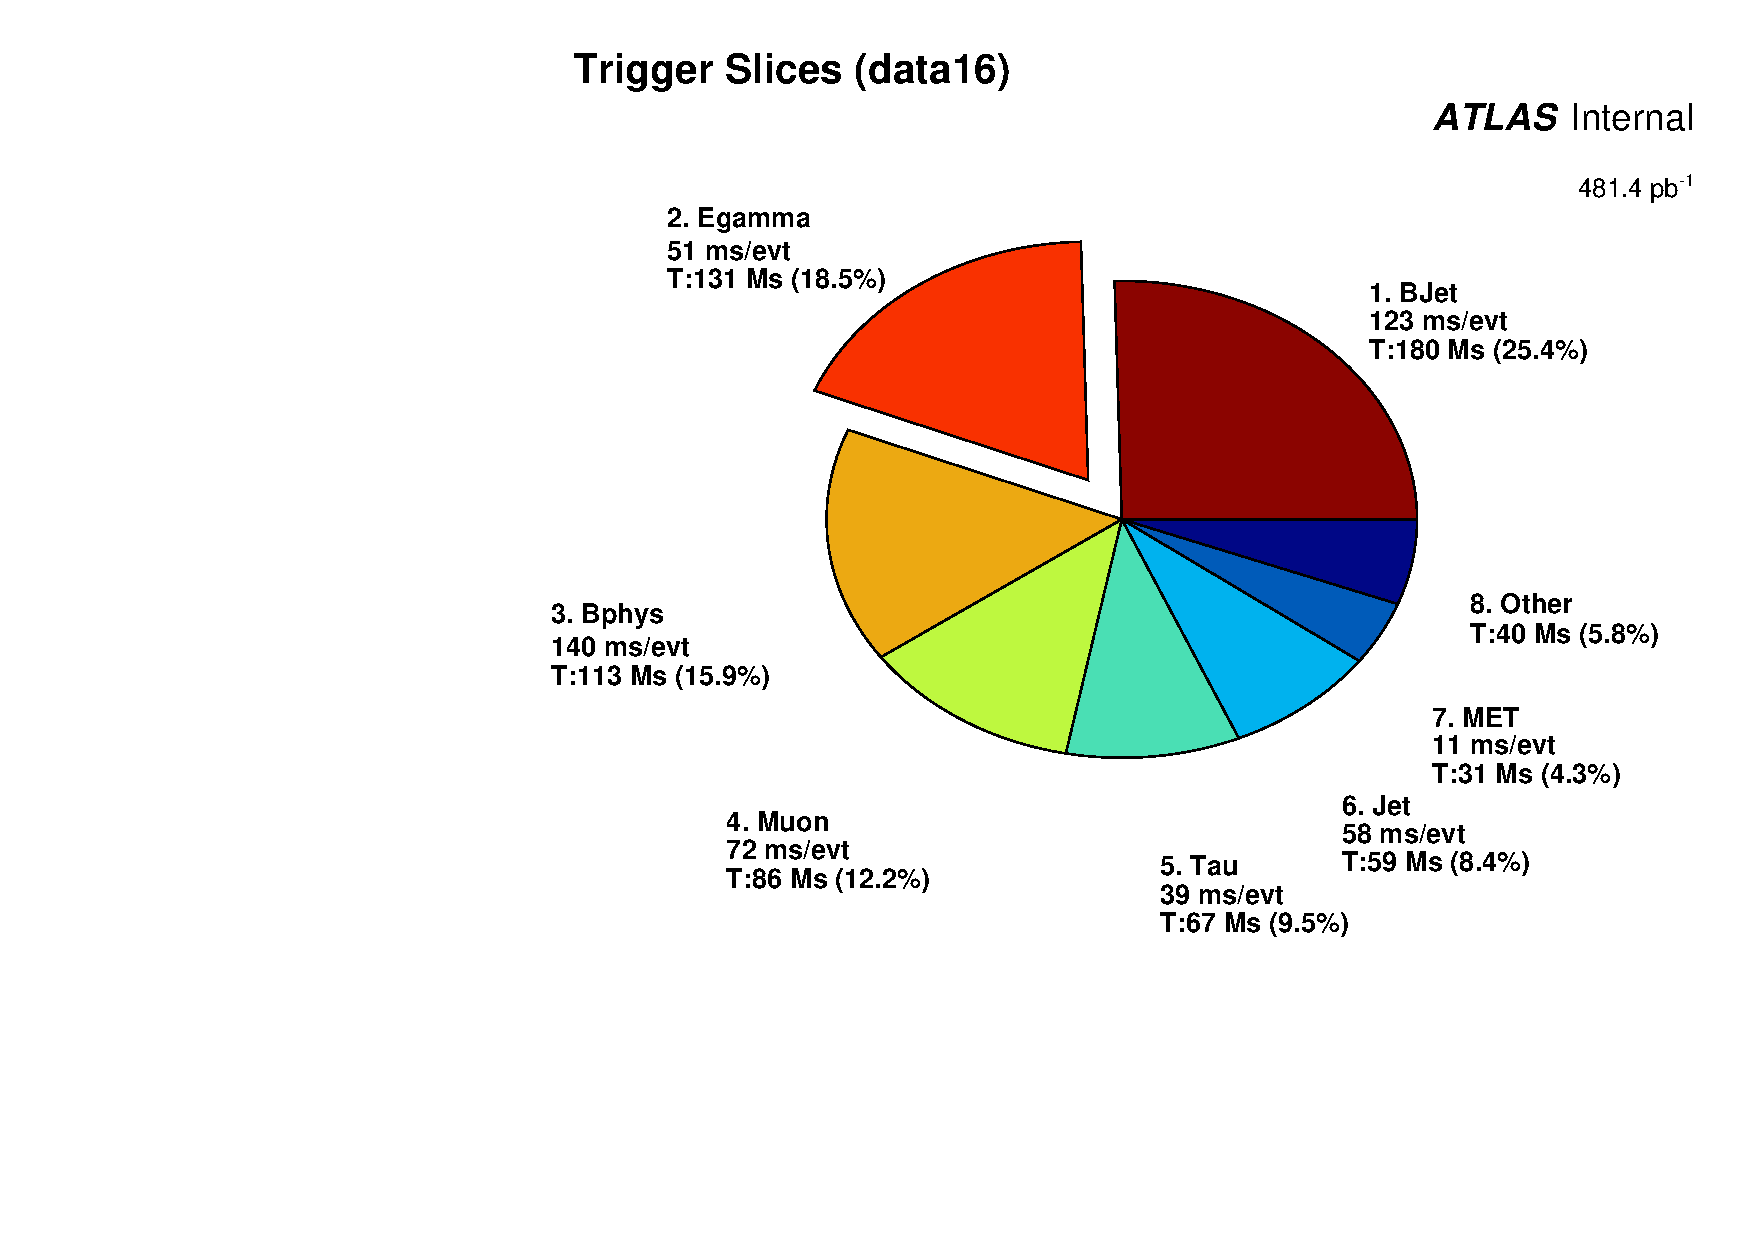
\includegraphics[width=\textwidth]{appendices/figures/menu_cpu_measurements/run2_slice_cpu_slices_pie_data16.pdf}
\caption{}%
\label{fig:run2_monitored_cpu_per_group_data16}
\end{subfigure}
\hfill
%\hspace{0.01\textwidth}
\begin{subfigure}[c]{.48\textwidth}
  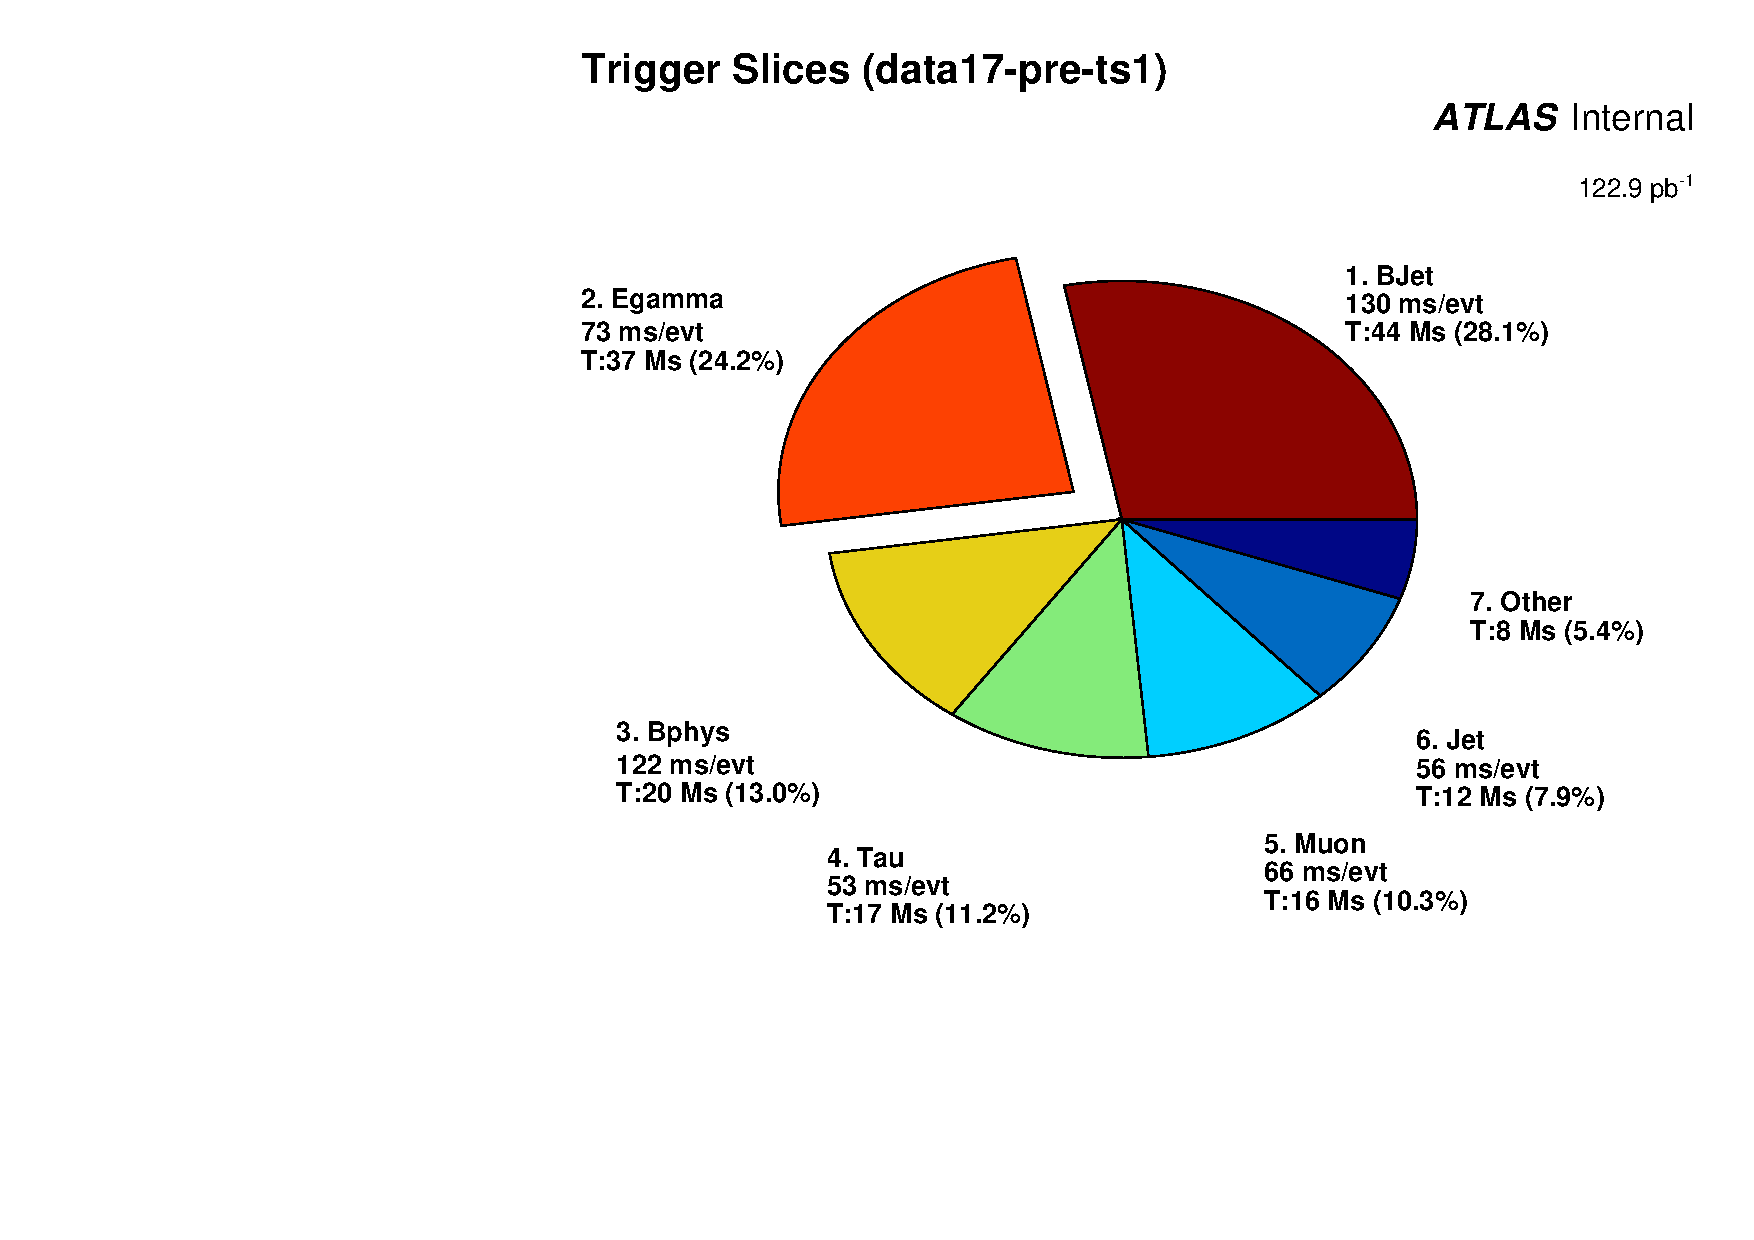
\includegraphics[width=\textwidth]{appendices/figures/menu_cpu_measurements/run2_slice_cpu_slices_pie_data17-pre-ts1.pdf}
\caption{}%
\label{fig:run2_monitored_cpu_per_group_data17_pre}
\end{subfigure} \\
\begin{subfigure}[c]{.48\textwidth}
  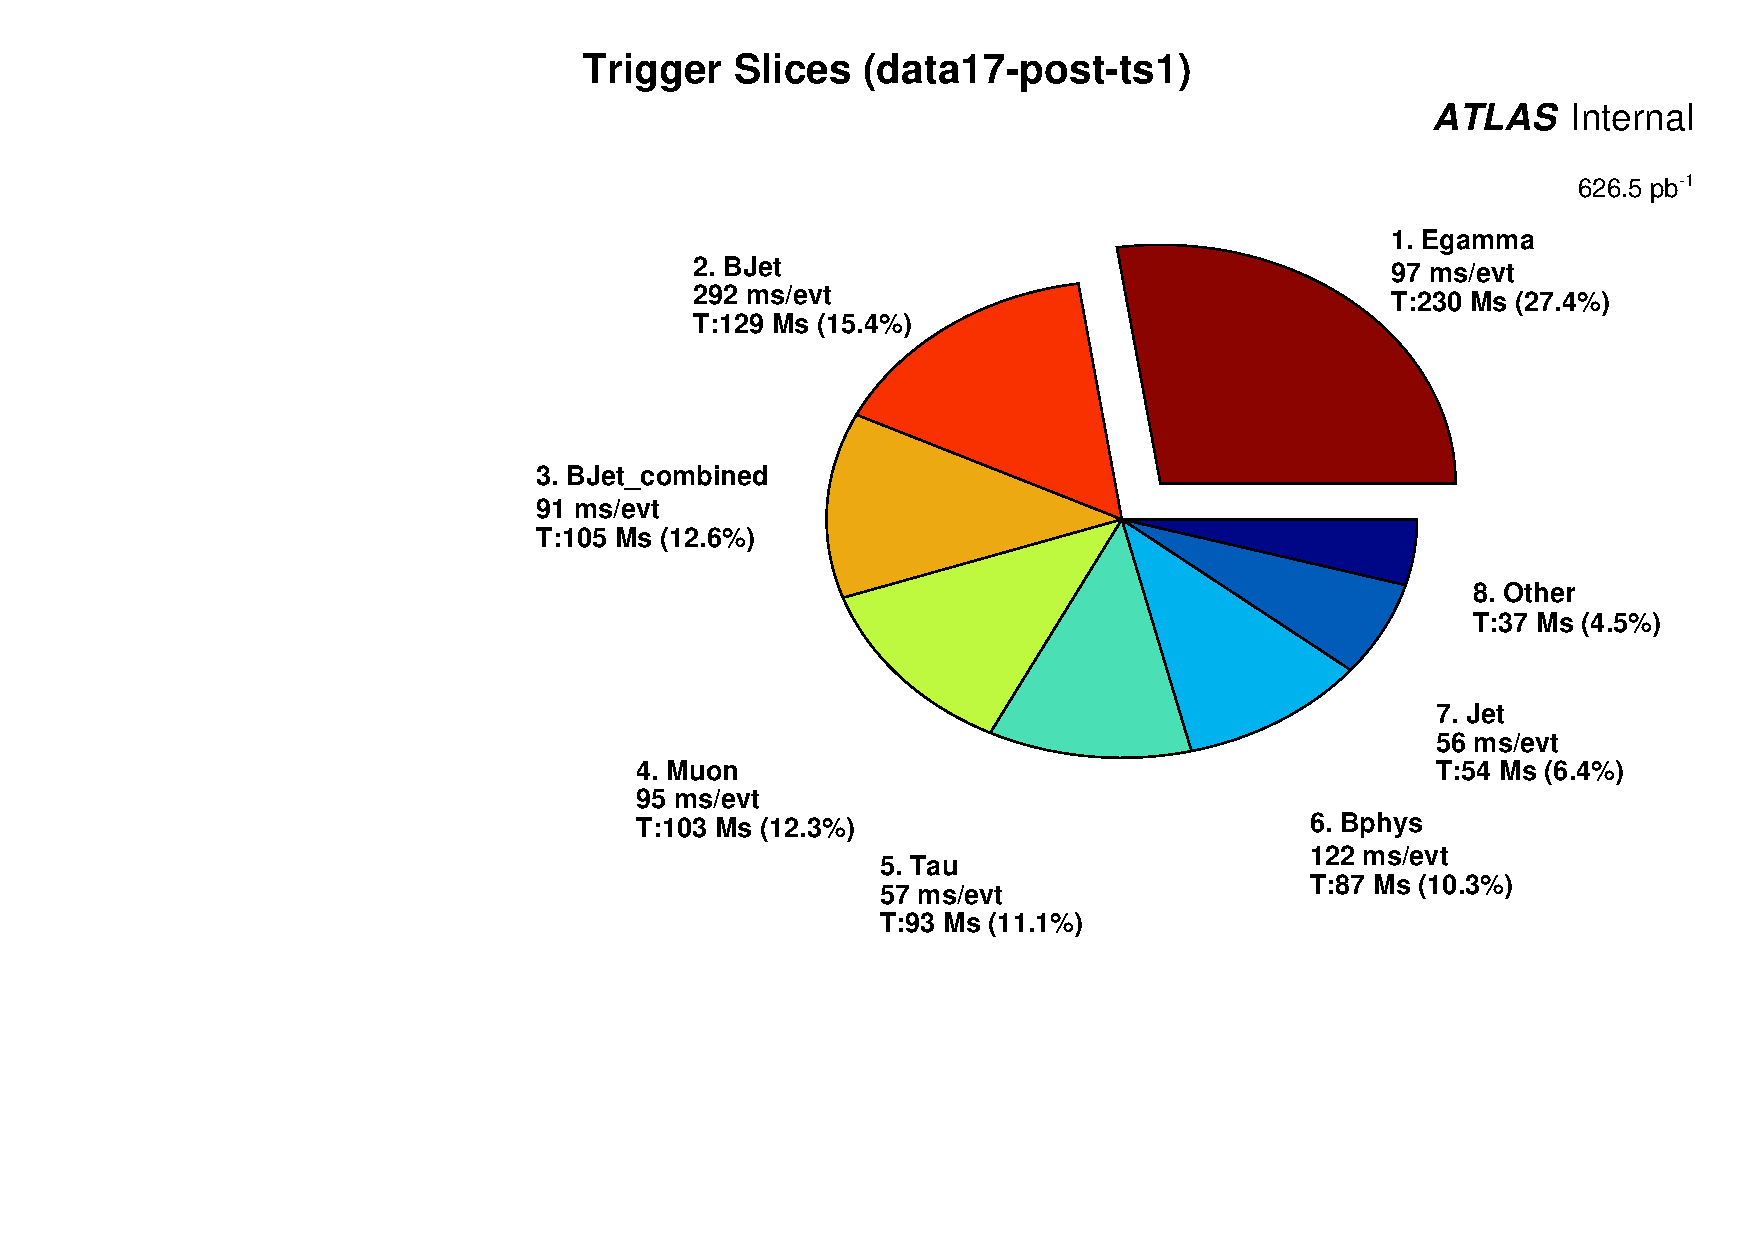
\includegraphics[width=\textwidth]{appendices/figures/menu_cpu_measurements/run2_slice_cpu_slices_pie_data17-post-ts1.pdf}
\caption{}%
\label{fig:run2_monitored_cpu_per_group_data17_post}
\end{subfigure} 
\begin{subfigure}[c]{.48\textwidth}
  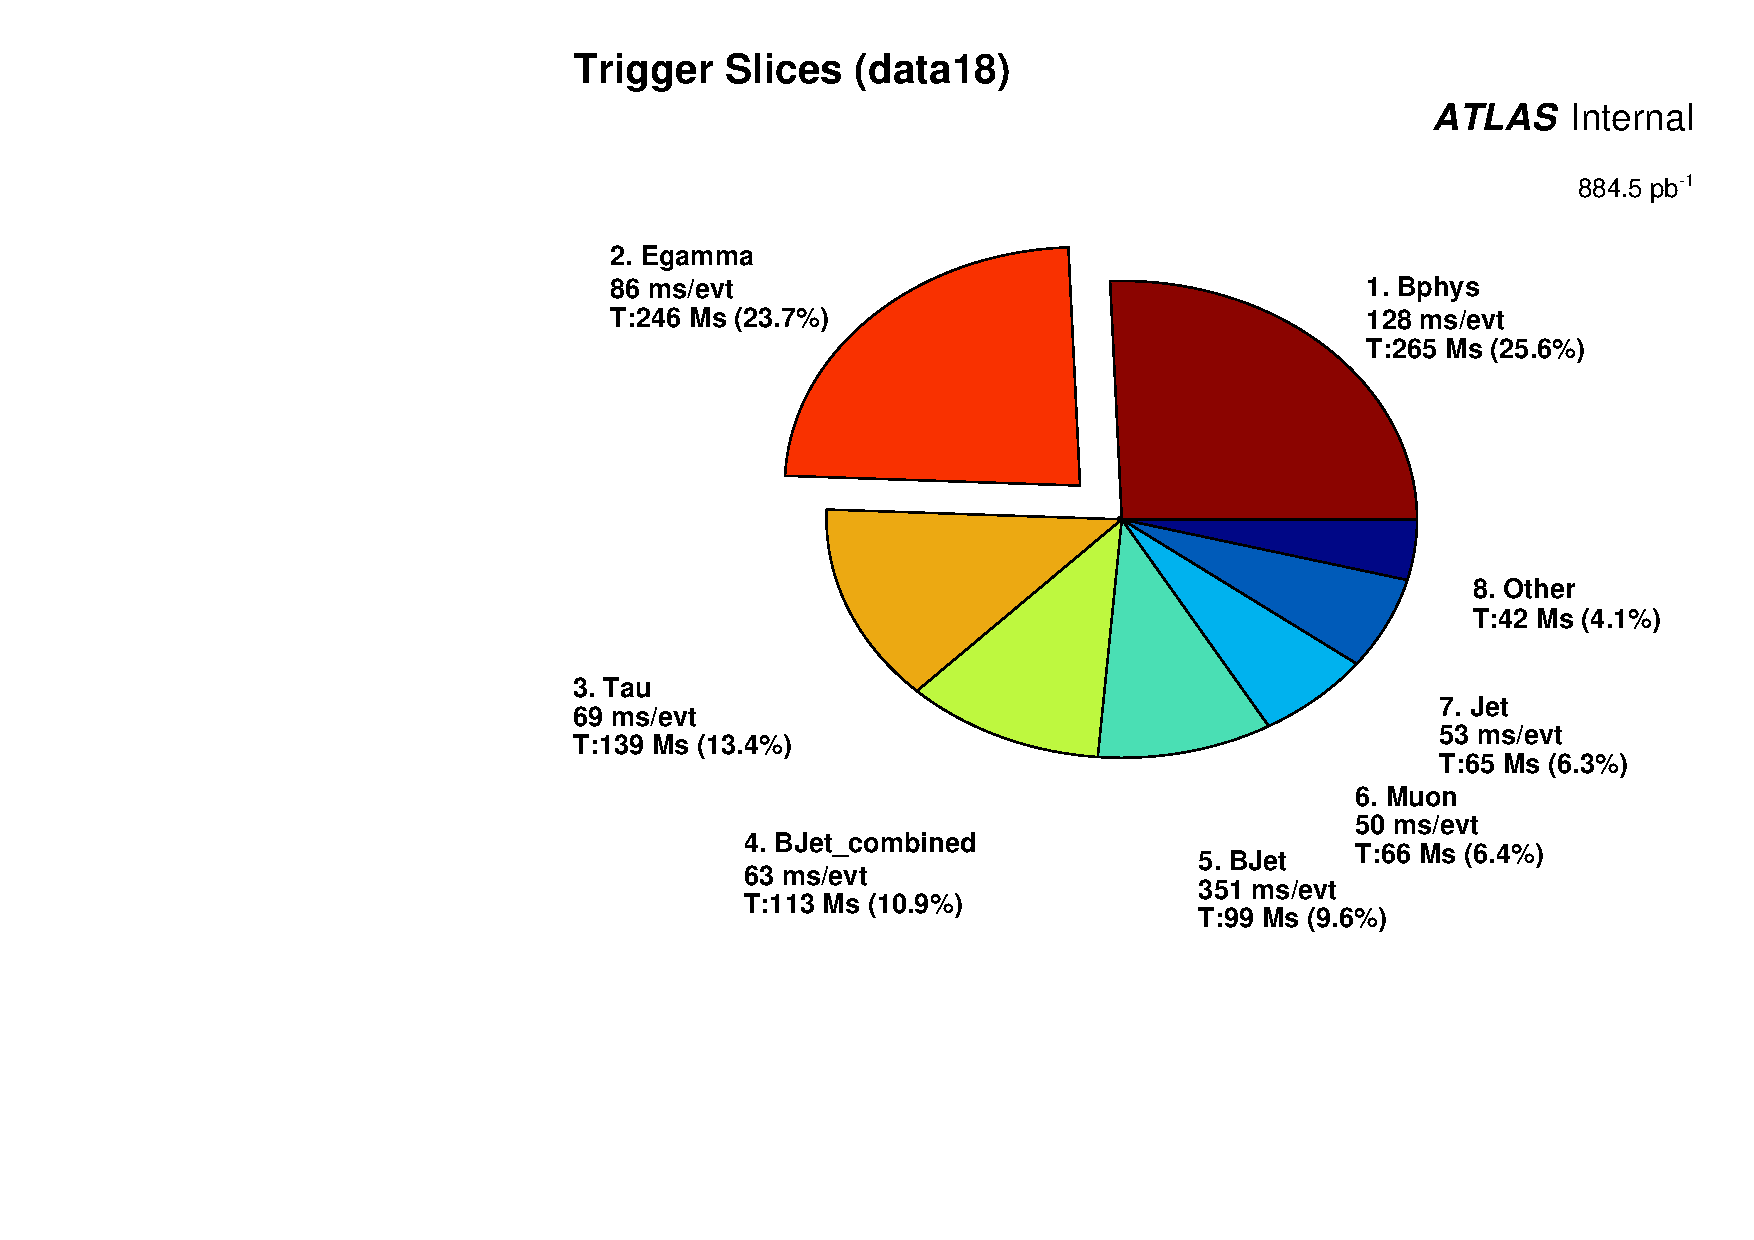
\includegraphics[width=\textwidth]{appendices/figures/menu_cpu_measurements/run2_slice_cpu_slices_pie_data18.pdf}
\caption{}%
\label{fig:run2_monitored_cpu_per_group_data18}
\end{subfigure} 
\caption{\label{fig:run2_monitored_cpu_per_group}CPU time demanded by each
  group. 2016 data are shown in (a), before 2017 TS1 in (b), after 2017 TS1 in
  (c) and 2018 in (d). The groups are in decreasing order based on the
  total CPU time demanded during the cost monitoring samplings. Emphasis is
  given in the graph to the \egamma{} group. Each group total time is displayed
  in the third line after for each group followed by the fraction of when
  considering the full HLT CPU time. The average CPU time per all HLT processed
  events is shown in the second line.
}
\end{figure}

\begin{figure}[h!tb]
\centering
\begin{subfigure}[c]{.48\textwidth}
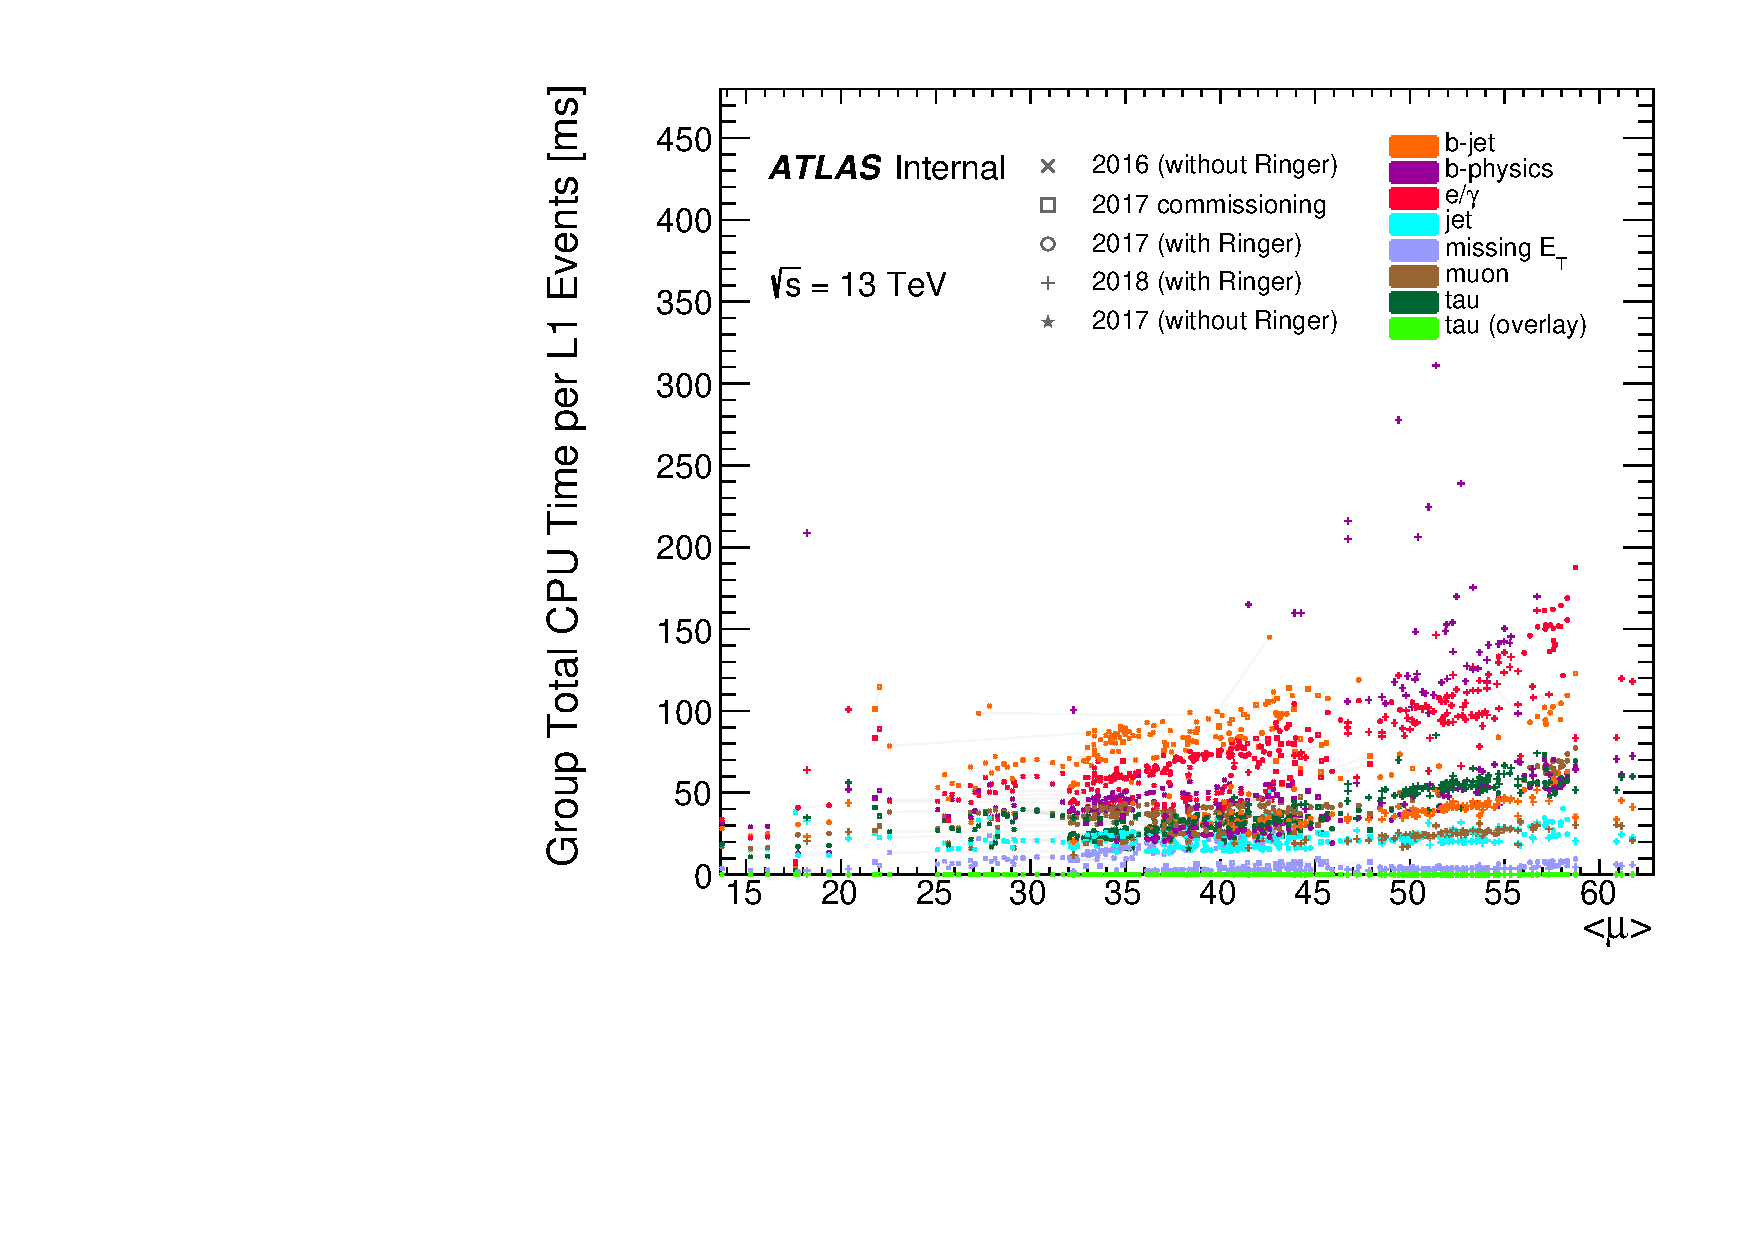
\includegraphics[width=\textwidth]{appendices/figures/menu_cpu_measurements/run2_slice_cpu_total_all_data.pdf}
\caption{}%
\label{fig:run2_monitored_cpu_per_mu_norm_l1_evt}
\end{subfigure}
\hfill
%\hspace{0.01\textwidth}
\begin{subfigure}[c]{.48\textwidth}
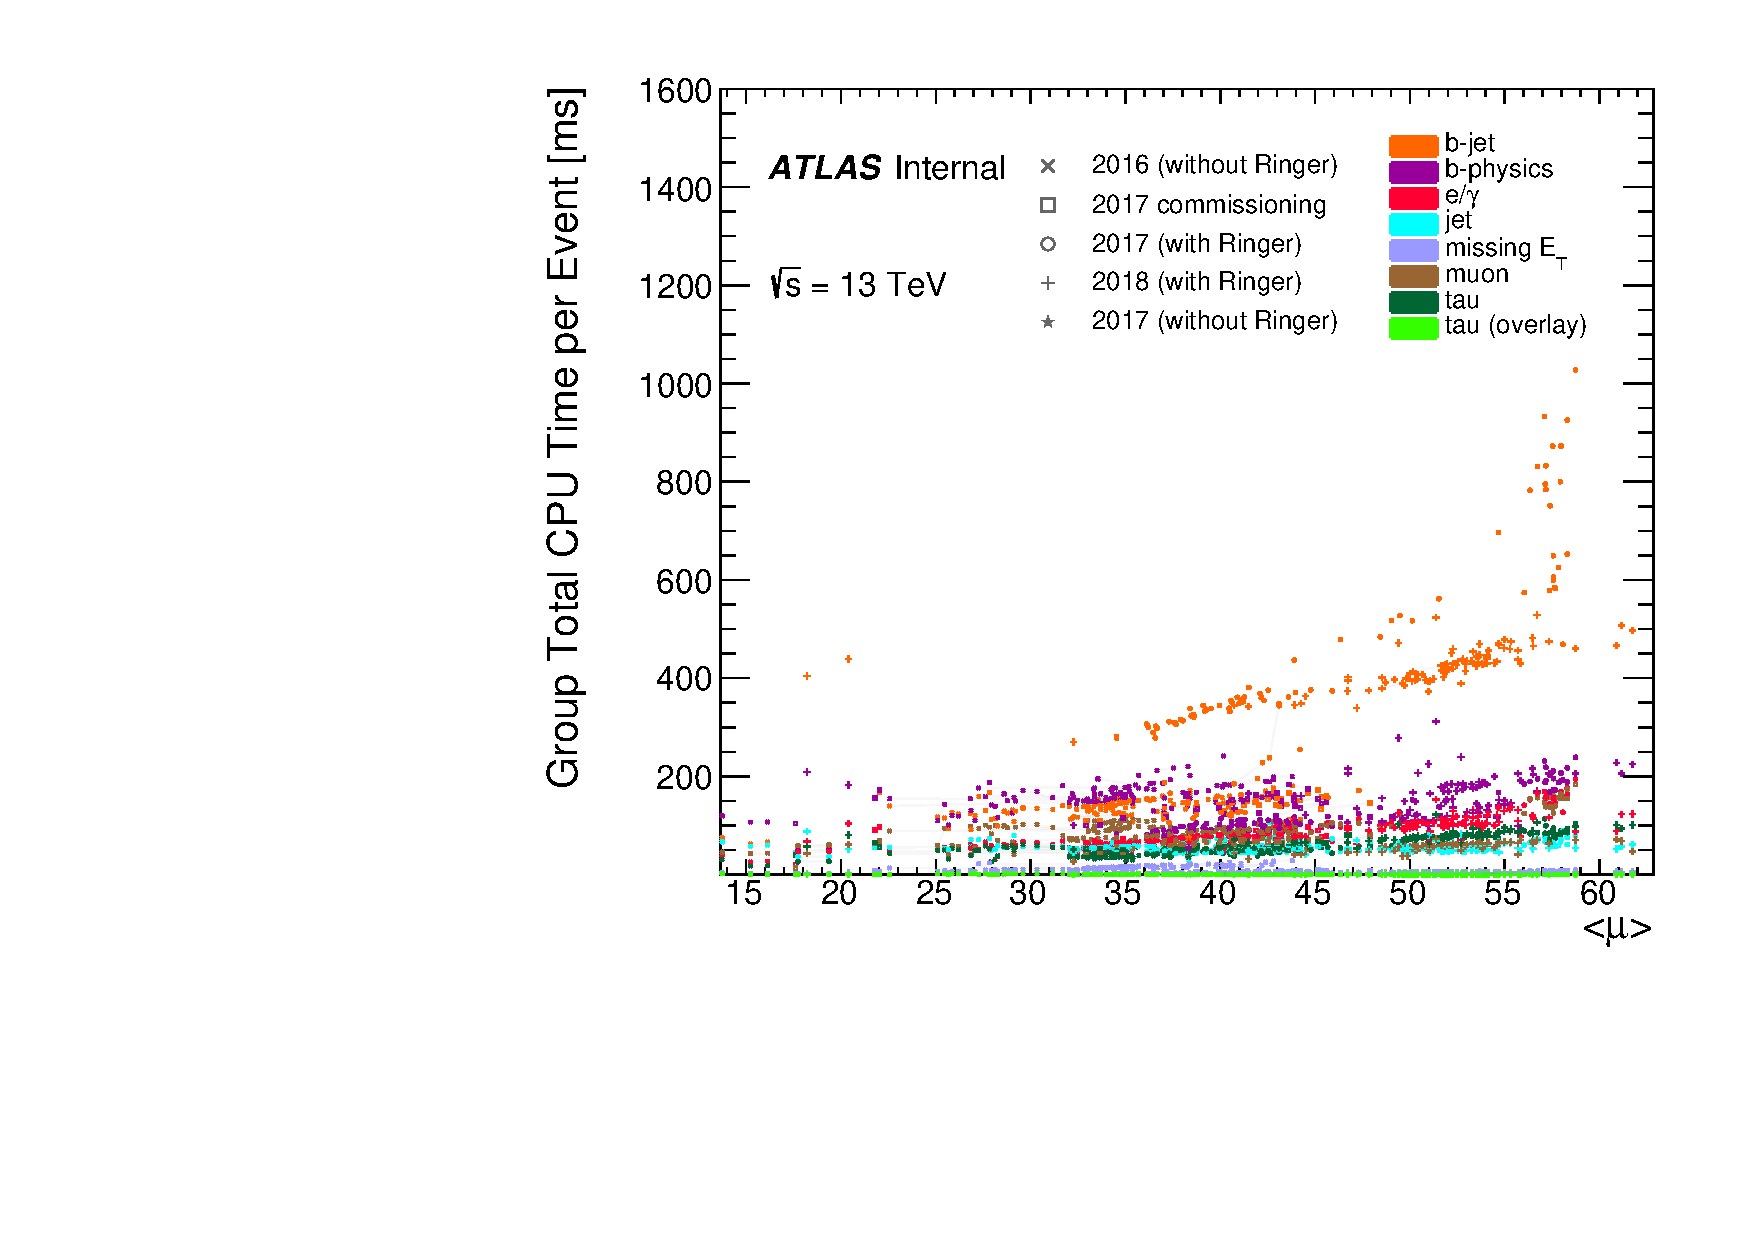
\includegraphics[width=\textwidth]{appendices/figures/menu_cpu_measurements/run2_slice_cpu_time_per_event_all_data.pdf}
\caption{}%
\label{fig:run2_monitored_cpu_per_mu_norm_group_evt}
\end{subfigure} \\
\caption{\label{fig:run2_monitored_cpu_per_mu}CPU time normalized by the
total number of L1 output (a) and each trigger signature events (b) as
function of \avgmu{}. The measurement colors are used to determine the signature
group and the marker style determine the period. 2016 data are shown with
crosses, before 2017 TS1 with squares, after 2017 TS1 with circles, 2018 with
plus marks and special data taking luminosity blocks during before 2017 TS1
configured without \rnn with stars. }
\end{figure}

Figure~\ref{fig:run2_monitored_egamma_cpu} shows the CPU demands according to
some trigger sub-groups within \egamma{}. Combined triggers refer to those that
require other physics object then the group they are placed in, i.e. an electron
trigger require a jet or a muon; as opposed to pure triggers. Additional
splitting is applied to electrons triggers depending on the energy of the
electron legs: a group for when all are above \SI{15}{\GeV} (affected by \rnn
operation after 2017 TS1); another for the case where all are below
\SI{15}{\GeV} (not affected); and a last group containing energy-thresholds at
both groups (partially affected by the \rnn).

\begin{figure}[h!tb]
\centering
\begin{subfigure}[c]{.48\textwidth}
  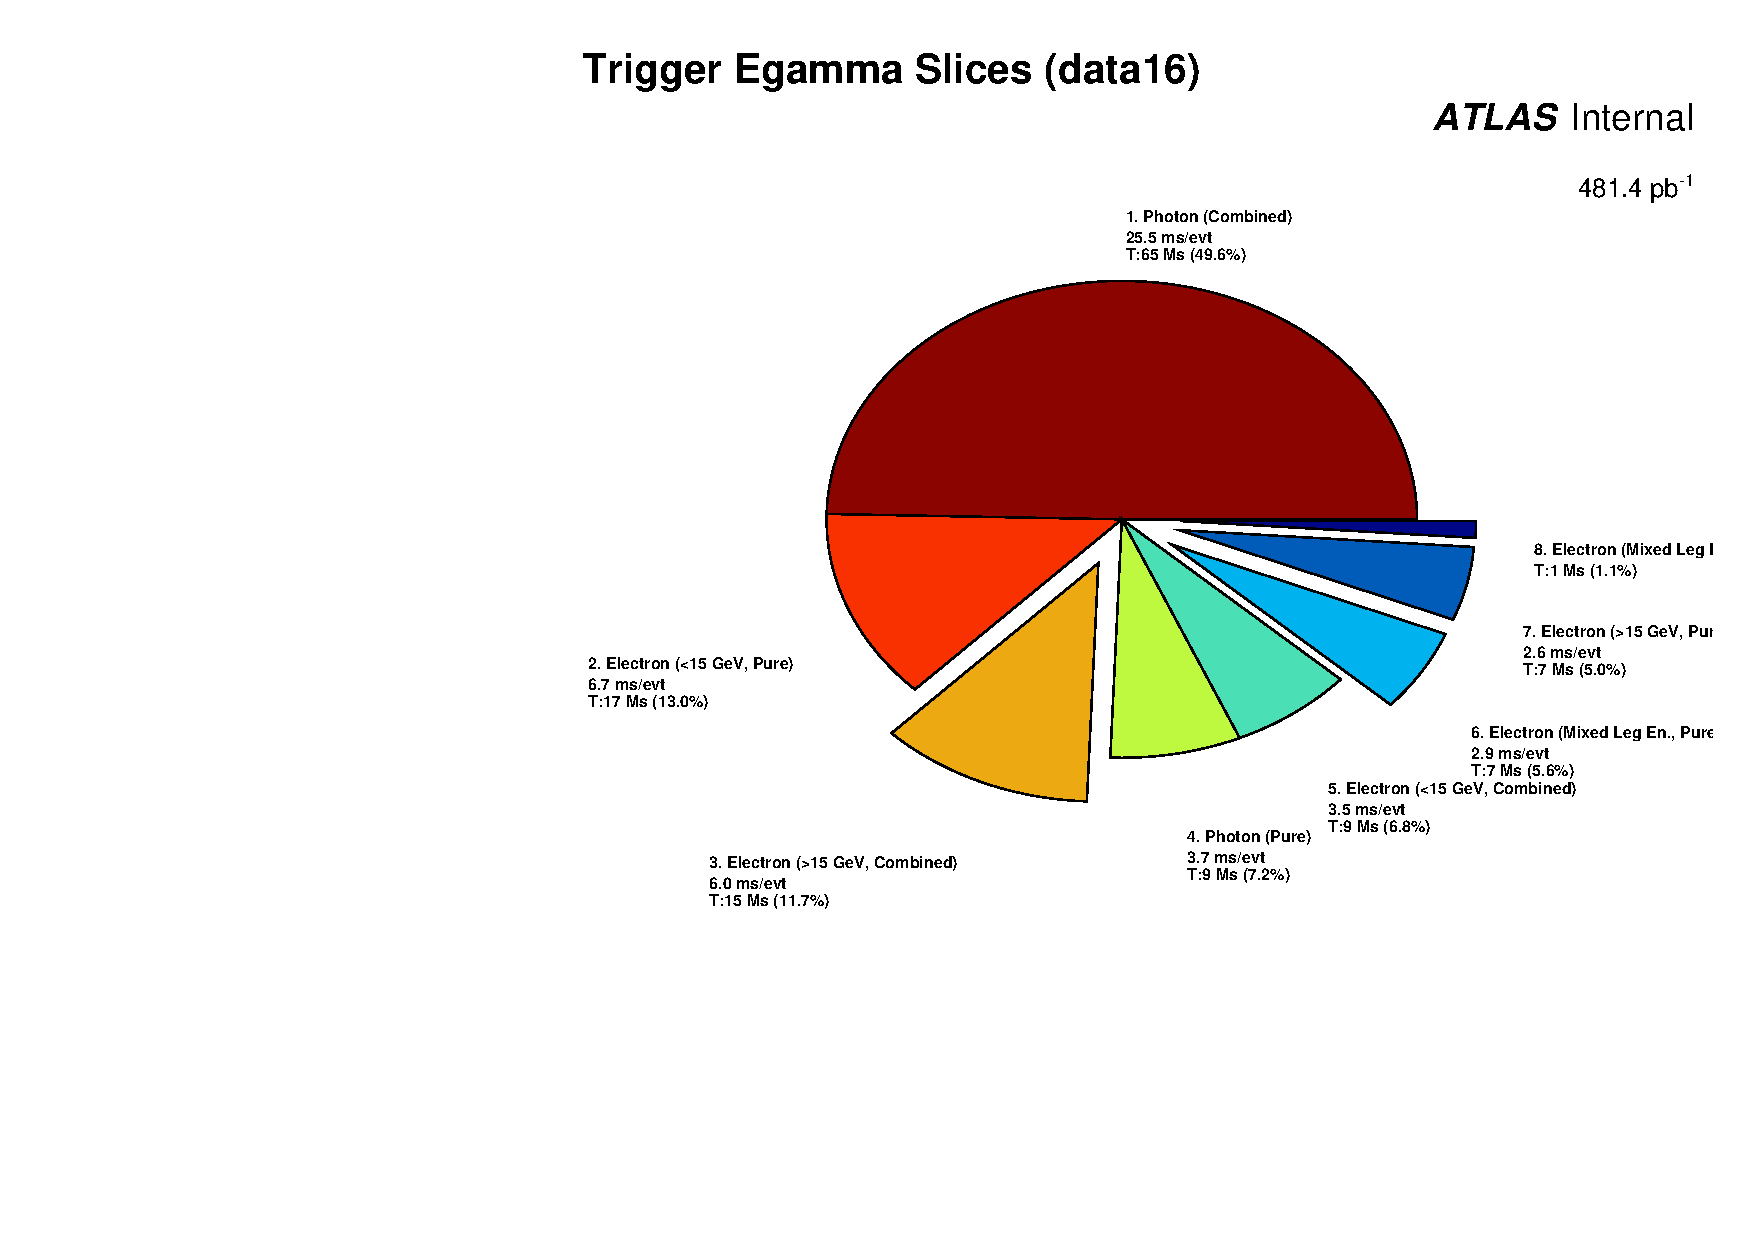
\includegraphics[width=\textwidth]{appendices/figures/menu_cpu_measurements/run2_slice_cpu_egamma_pie_data16.pdf}
\caption{}%
\label{fig:run2_monitored_egamma_cpu_data16}
\end{subfigure}
\hfill
%\hspace{0.01\textwidth}
\begin{subfigure}[c]{.48\textwidth}
  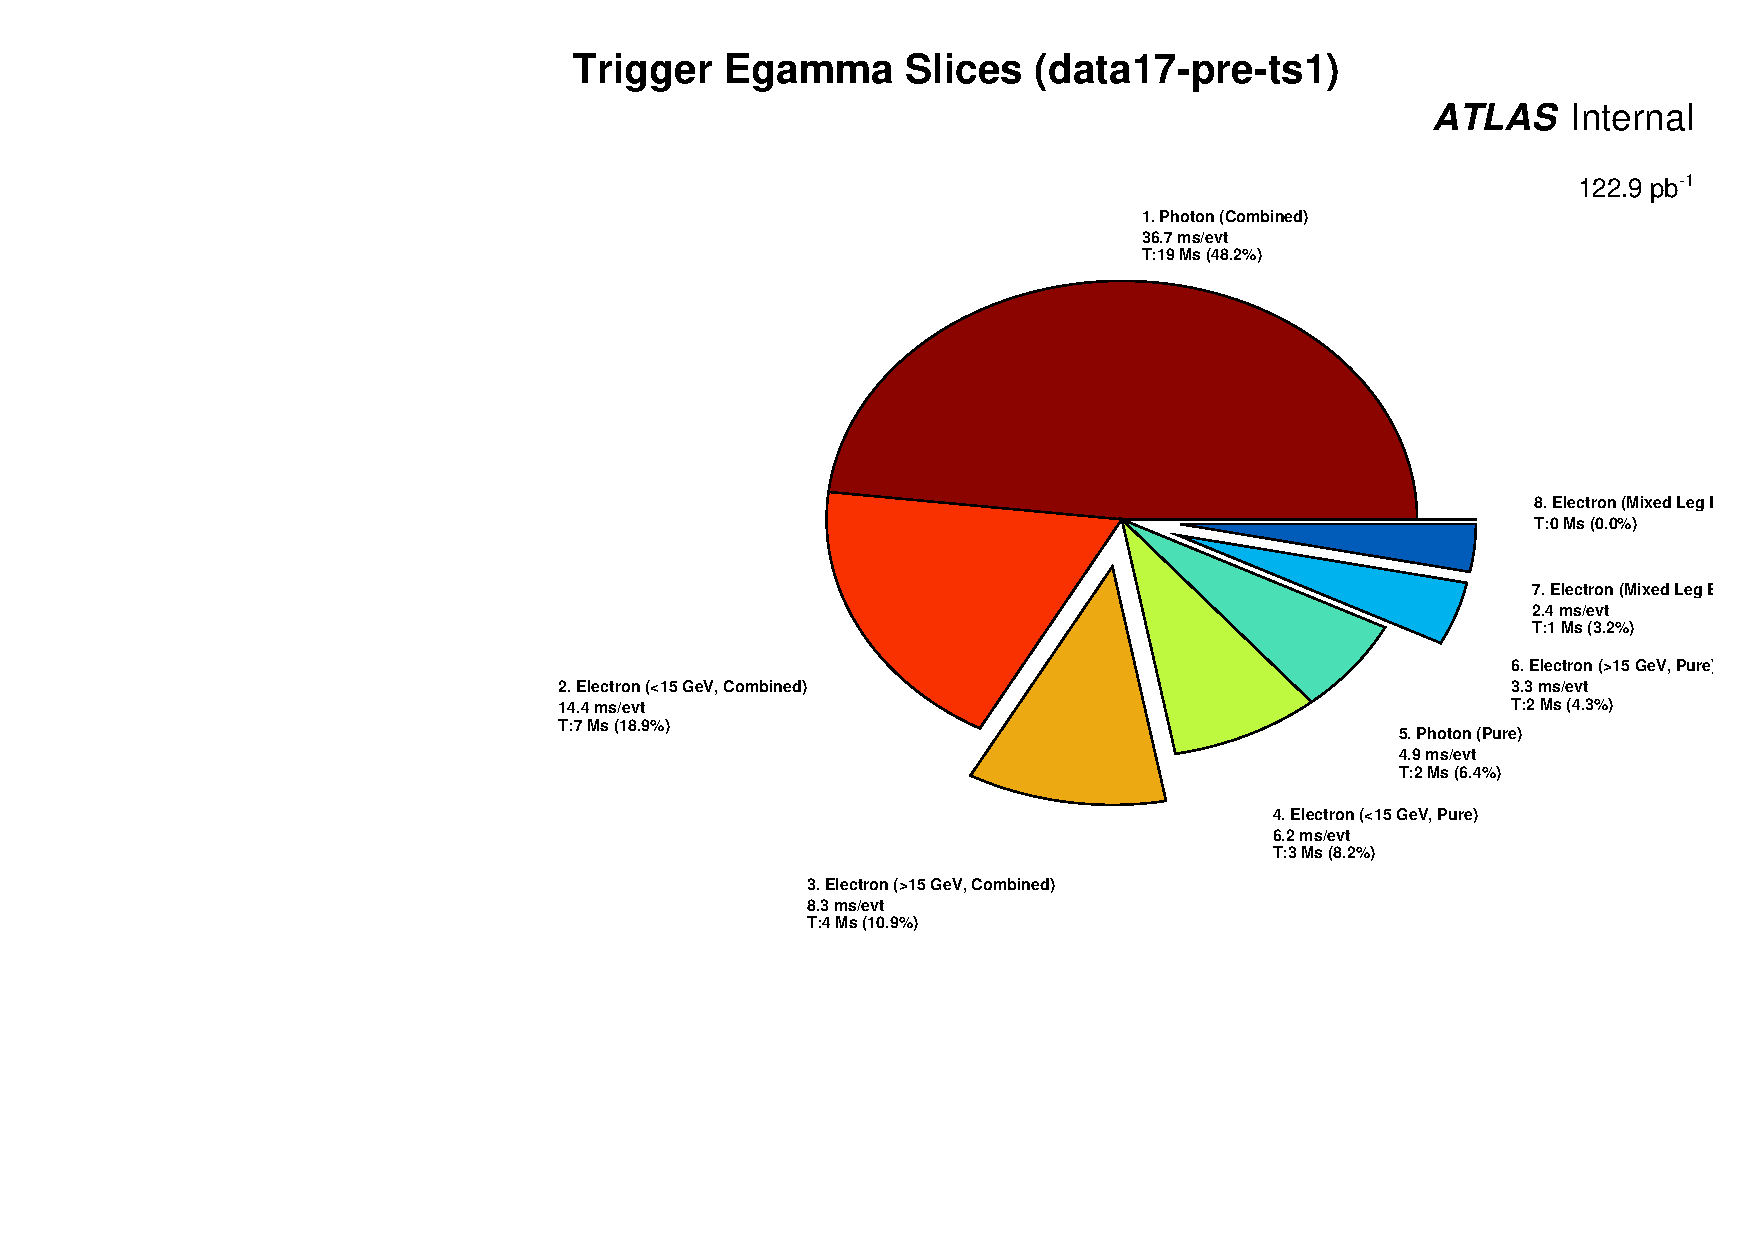
\includegraphics[width=\textwidth]{appendices/figures/menu_cpu_measurements/run2_slice_cpu_egamma_pie_data17-pre-ts1.pdf}
\caption{}%
\label{fig:run2_monitored_egamma_cpu_data17_pre}
\end{subfigure} \\
\begin{subfigure}[c]{.48\textwidth}
  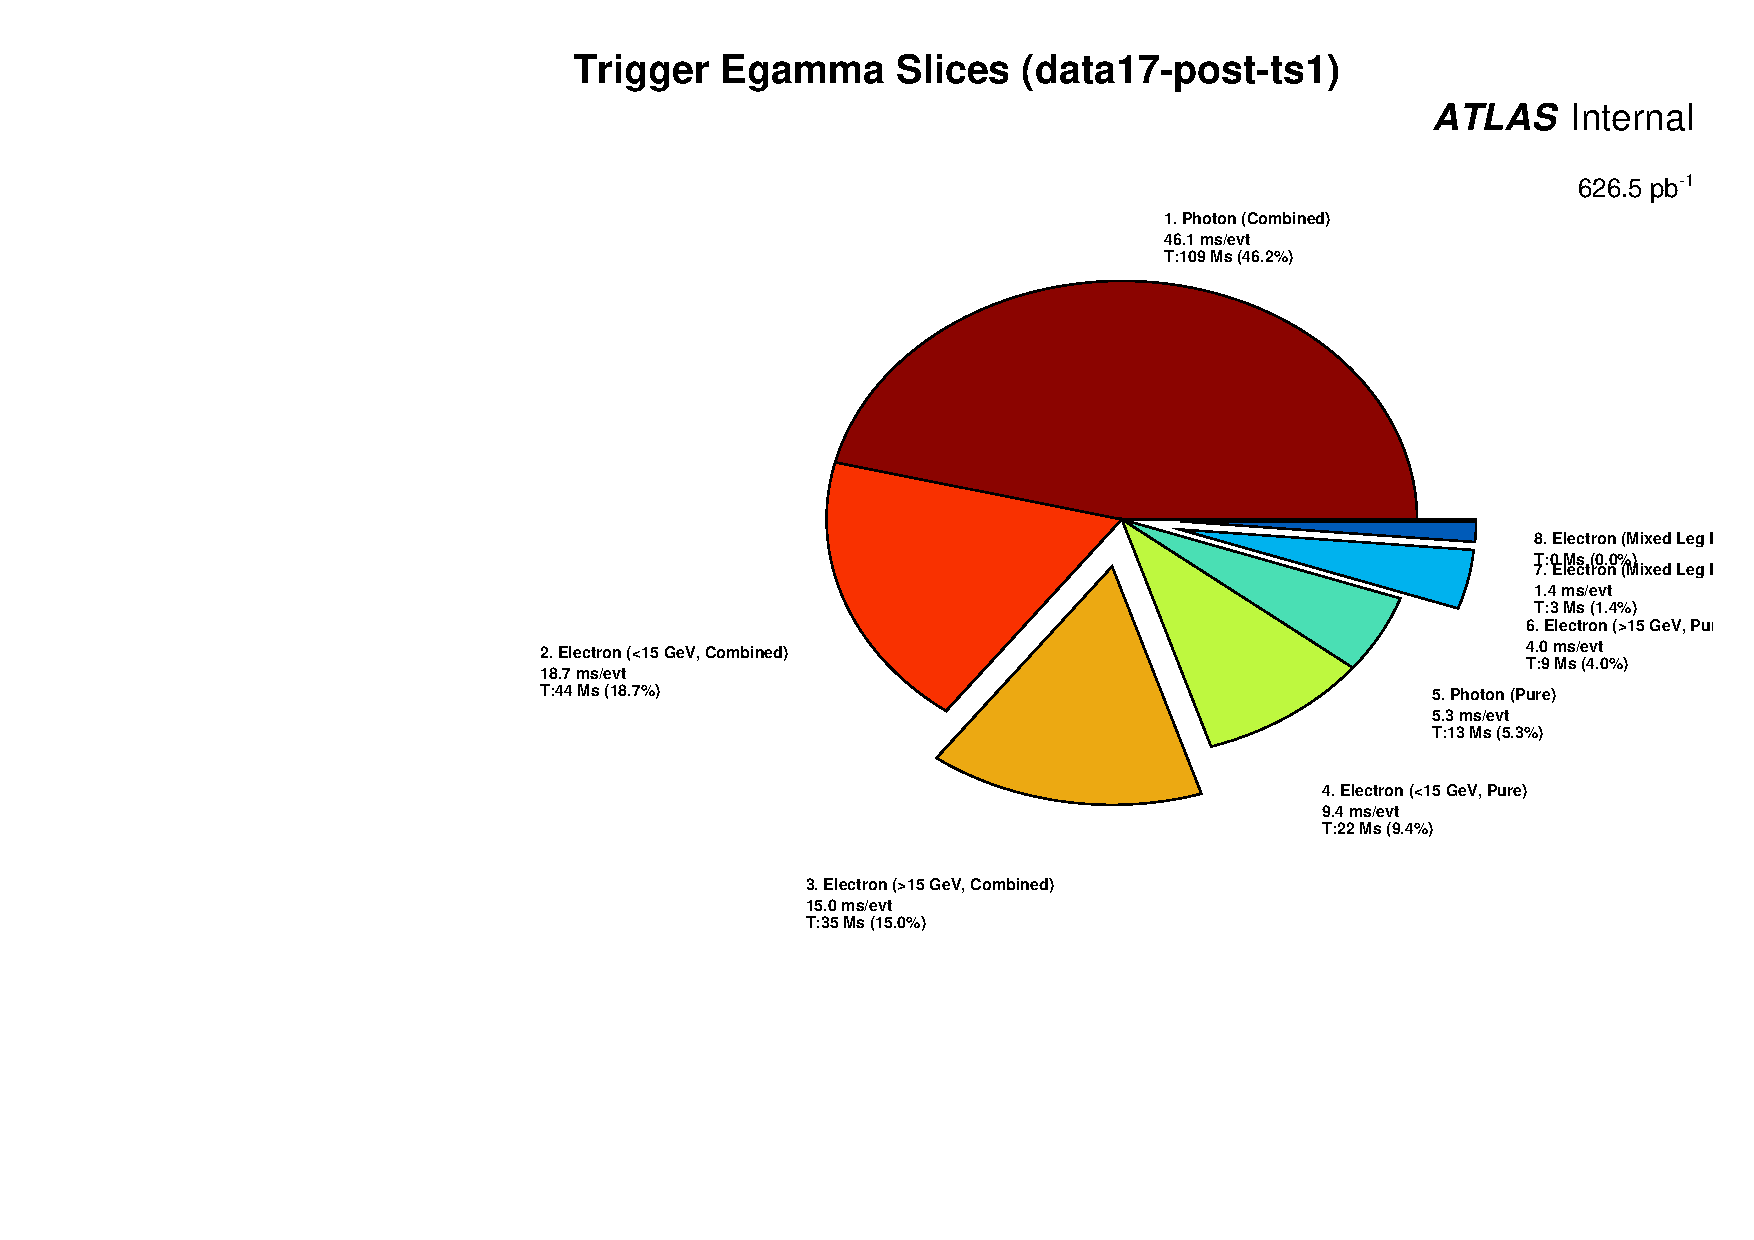
\includegraphics[width=\textwidth]{appendices/figures/menu_cpu_measurements/run2_slice_cpu_egamma_pie_data17-post-ts1.pdf}
\caption{}%
\label{fig:run2_monitored_egamma_cpu_data17_post}
\end{subfigure}
\begin{subfigure}[c]{.48\textwidth}
  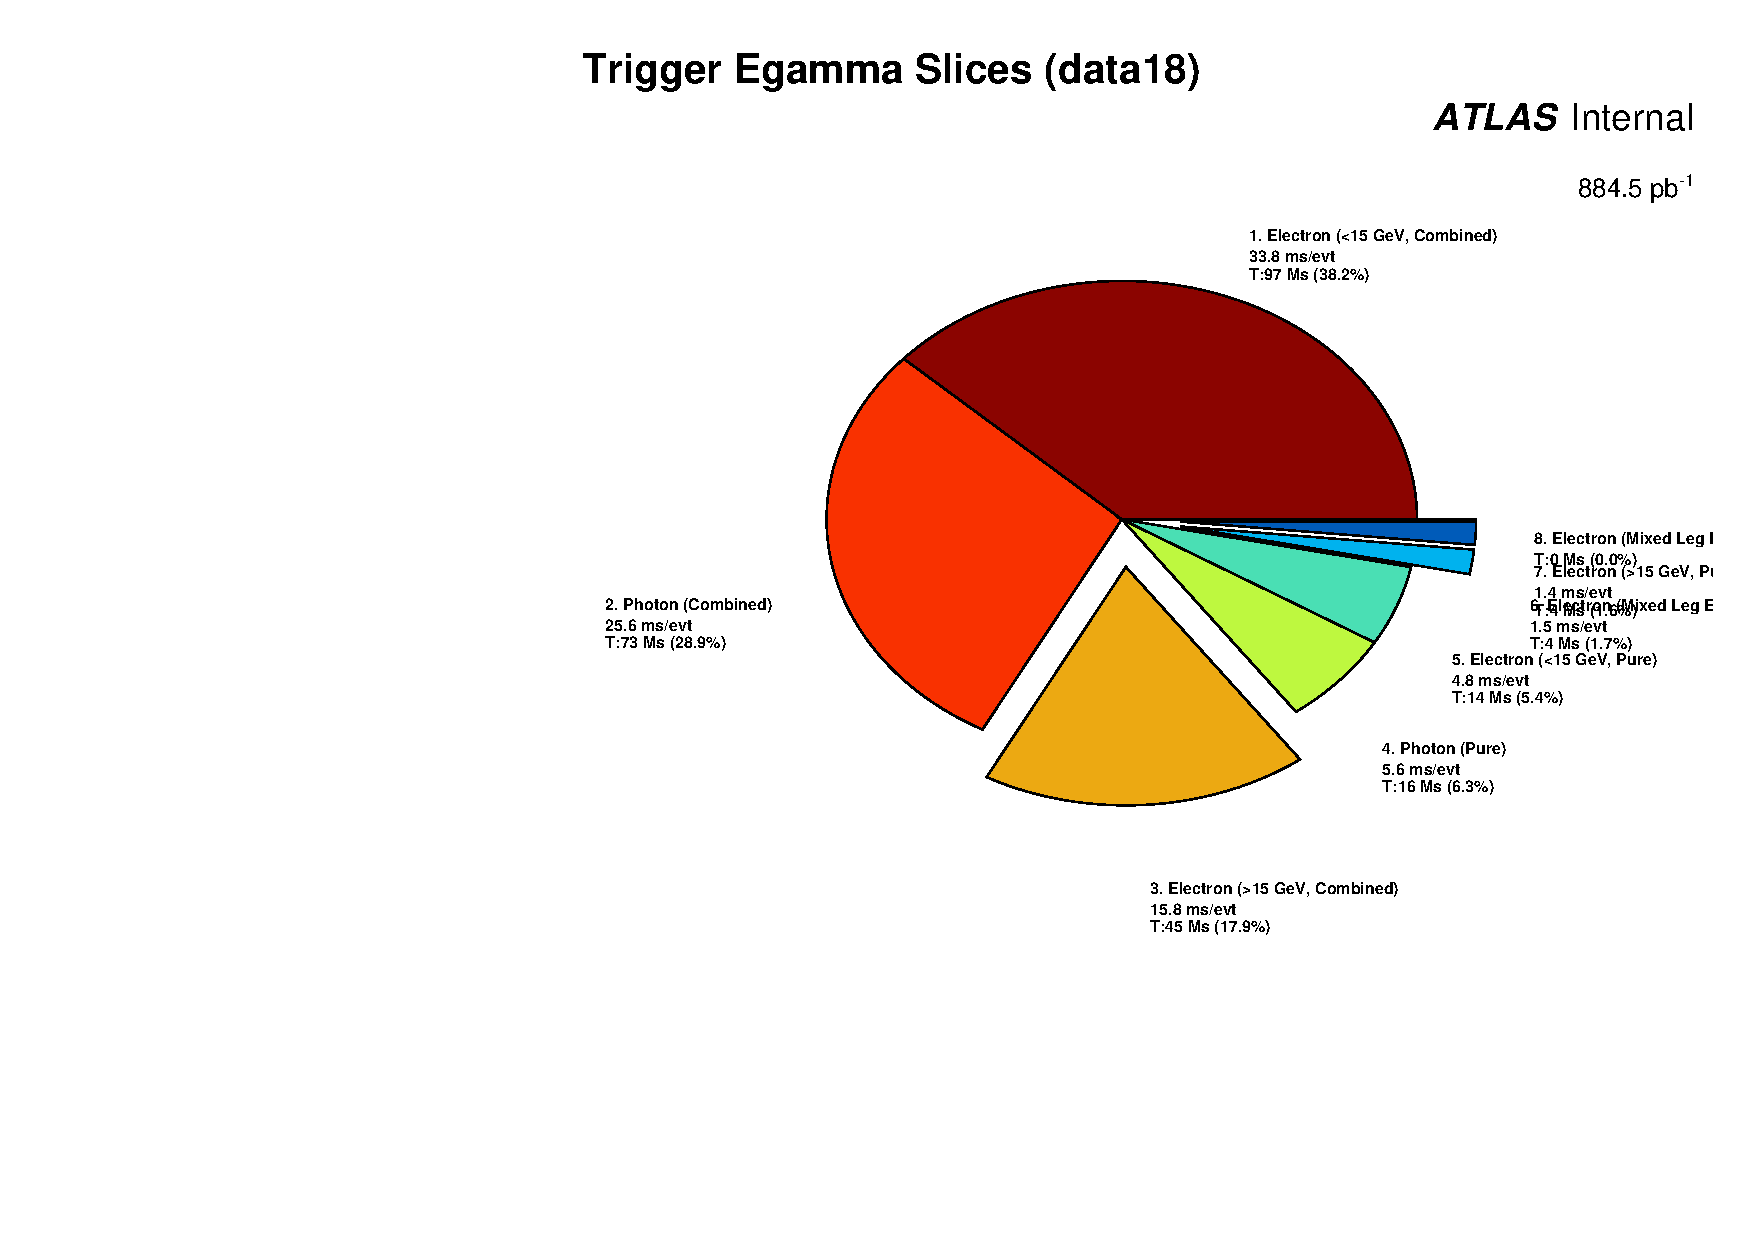
\includegraphics[width=\textwidth]{appendices/figures/menu_cpu_measurements/run2_slice_cpu_egamma_pie_data18.pdf}
\caption{}%
\label{fig:run2_monitored_egamma_cpu_data18}
\end{subfigure}
\caption{\label{fig:run2_monitored_egamma_cpu}CPU time demanded by
\egamma{} triggers grouped by the leg configurations. The groups are in
decreasing order based on the total CPU time demanded during the cost monitoring
samplings. The groups where \rnn changed the configuration during Run~2 are
dislocated with respect to the center. Emphasis is given in the graph to the
groups where \rnn{} changed the configuration during Run~2. Each group total
time is displayed in the third line after for each group followed by the
fraction of when considering the full HLT CPU time. The average CPU time per all
HLT processed events is shown in the second line.
}
\end{figure}

The most demanding \egamma{} sub-groups are combined photon triggers and
combined electron triggers with legs below \SI{15}{\GeV}. Together, they demand
around $2/3$ of the \egamma{} group CPU. When considering pure photon triggers
and combined electron triggers to take all groups unaffected by the \rnn
operation during Run~2, fraction goes to nearly $3/4$ of the \egamma{} CPU.\@
Hence, there is a great potential for the \rnn{} to further release resources in
next data-takings by enabling its operation for these other groups, namely
triggers with electron legs below \SI{15}{\GeV} and photon combined triggers.

To have an idea of the fraction of P1 CPU that could benefit of a
more efficient early selection as offered by the \rnn{}, we show the most CPU
demanding triggers containing at least an electron or a photon in
Table~\ref{tab:top_cpu_electrons} and Table~\ref{tab:top_cpu_photons},
respectively. It can be observed that these triggers alone required about
\SI{15}{\%} to \SI{30}{\%} of the total CPU during Run~2. Except for a few
triggers that do not apply any requirement in the electron or photon legs
(i.e.\@ the g0 and etcut triggers), the \rnn{} may be able to bring considerable
additional impact if set to operate on the electron and photon legs.

%As shown in Section~\ref{top:menu_cpu}, a great potential for saving CPU is
%available if the \rnn{} is developed for selecting electrons with
%$\et<\SI{15}{\GeV}$. Additionally, as many of those triggers are prescaled to
%reduce their output rate in addition to the CPU limitations, it is possible that
%the \rnn{} algorithm can allow to reduce the pre-scale factor if it is capable
%of impacting the \hlt{} fake rate as it was the case of the factor of
%\SI{2}{$\times$} reduction for the duplicated trigger during 2017
%(Section~\ref{ssec:2017_ringer_operation}).

\FloatBarrier

\begin{table}[!ht]
    \centering
    \caption{\label{tab:top_cpu_electrons}Most-demanding electron triggers using
    Run 2 cost-monitoring data. The triggers are sorted out in decreasing order
    using the integrated CPU time (in seconds), while the CPU demands are shown in
    percentage when considering the total P1 CPU processing time in cost
    monitorings. Before TS1 data are labelled as {data17-}, whereas {data17+}
    dedicates to the remaining 2017 runs.}
    \resizebox{\textwidth}{!}{%
      \begin{tabular}{p{20cm}cccc}
    \hline\hline
    Trigger with at least one electron leg & \multicolumn{4}{c}{P1 Total Trigger Time [\%]} \\
    \hline
    data type&
    data16 &
    data17-&
    data17+&
    data18 \\
    \hline
    HLT\_e60\_etcut\_trkcut\_L1EM24VHIM\_xs30\_j15\_perf\_xe30\_6dphi15\_mt35&
    &
    &
    2.48&
    2.81 \\
    HLT\_e7\_lhmedium\_nod0\_mu24&
    0.82&
    1.31&
    1.62&
    1.98 \\
    HLT\_e9\_lhvloose\_nod0\_mu20\_mu8noL1\_L1EM7\_MU20&
    &
    &
    &
    2.19 \\
    HLT\_mu20\_mu8noL1\_e9\_lhvloose\_nod0&
    &
    1.19&
    1.27&
    1.76\\
    HLT\_e5\_lhmedium\_nod0\_j40\_xe80\_pufit\_2dphi10\_L1XE60&
    &
    1.79&
    &
    \\
    HLT\_mu20\_mu8noL1\_e9\_lhvloose\_nod0\_L1EM7\_MU20&
    &
    1.95&
    2.01&
    2.65\\
    HLT\_e5\_lhloose\_nod0\_j40\_xe70\_pufit\_2dphi10\_L1XE60&
    &
    0.25&
    1.28&
    1.08 \\
    HLT\_e9\_lhvloose\_nod0\_mu20\_mu8noL1&
    &
    &
    &
    1.35 \\
    HLT\_e5\_lhmedium\_nod0\_j50\_xe80\_\_2dphi10\_L1J40\_XE50\_DPHI-J20s2XE50pufit&
    &
    0.51&
    0.69&
    0.82 \\
    HLT\_e5\_lhtight\_nod0\_e14\_etcut\_Jpsiee\_L1JPSI-1M5-EM12&
    &
    &
    2.44&
    1.53 \\
    HLT\_e28\_lhtight\_nod0\_noringer\_ivarloose\_L1EM24VHIM&
    &
    &
    0.56&
    \\
    HLT\_e5\_lhloose\_nod0\_mu4\_j30\_xe40\_pufit\_2dphi10\_L1MU4\_J30\_XE40\_DPHI-J20s2XE30&
    &
    0.34&
    0.50&
    0.55 \\
    HLT\_e28\_lhtight\_nod0\_L1EM24VHIM\_e15\_etcut\_L1EM7\_Zee&
    &
    0.59&
    0.28&
    0.30 \\
    HLT\_e26\_lhmedium\_nod0\_mu8noL1&
    &
    0.18&
    0.11&
    0.47 \\
    HLT\_e5\_lhtight\_nod0\_e14\_etcut\_Jpsiee&
    &
    0.91&
    2.3&
     \\
    HLT\_e5\_lhtight\_nod0 (rerun)&
    0.28&
    0.39&
    0.36&
    0.40 \\
    HLT\_e26\_lhtight\_nod0\_e15\_etcut\_L1EM7\_Zee&
    0.53&
    0.02&
    0.02&
    0.07 \\
    HLT\_2e5\_lhmedium\_nod0\_j70\_j50\_0eta490\_invm900j50\_L1MJJ-700&
    &
    &
    &
    0.64 \\
    HLT\_e26\_lhmedium\_nod0\_L1EM22VHIM\_mu8noL1&
    &
    0.42&
    0.34&
    \\
    HLT\_e13\_etcut\_trkcut\_L1EM12&
    0.44&
    0.30&
    &
    \\
    HLT\_e28\_lhmedium\_nod0\_L1EM24VHIM\_mu8noL1&
    &
    0.04&
    0.02&
    0.02 \\
    HLT\_2e5\_lhmedium\_nod0\_j70\_j50\_0eta490\_invm900j50\_L1MJJ-500-NFF &
    &
    &
    &
    0.52 \\
    HLT\_e5\_lhtight\_nod0\_e9\_etcut\_Jpsiee\_L1JPSI-1M5-EM7 &
    &
    &
    0.94&
    0.56 \\
    HLT\_e14\_etcut\_e5\_lhtight\_nod0\_Jpsiee &0.67& & & \\
    HLT\_e13\_etcut\_trkcut\_xs30\_j15\_perf\_xe30\_6dphi15\_mt35 &
    0.14& 0.29& 0.34& 0.29 \\
    \hline
    Total& 2.89 & 10.47 & 17.64 & 20.10\\
    \hline
    \hline
    \end{tabular}
    }
    \end{table}
    
\begin{table}[!ht]
    \centering
    \caption{\label{tab:top_cpu_photons}Most-demanding photon triggers using
    Run 2 cost-monitoring data. Trigger and CPU information as in
    Table~\ref{tab:top_cpu_electrons}.}
    \resizebox{\textwidth}{!}{%
      \begin{tabular}{p{20cm}cccc}
    \hline\hline
    Trigger with at least one photon leg & \multicolumn{4}{c}{P1 Total Trigger Time [\%]} \\
    \hline
    data type&
    data16 &
    data17-&
    data17+&
    data18 \\
    \hline
    HLT\_g27\_medium\_L1EM24VHI\_2j15\_gsc35\_bmv2c1077\_split\_2j35\_0eta490&
    4.21&
    4.81&
    \\
    HLT\_g35\_loose\_L1EM24VHI\_mu15noL1\_mu2noL1&
    3.02&
    &
    &
    \\
    HLT\_g27\_medium\_L1EM24VHI\_2j35\_bmv2c1077\_split\_2j35\_0eta490&
    &
    &
    0.00&
    1.47\\
    HLT\_g40\_tight\_icalotight\_L1EM24VHI\_mu15noL1\_mu2noL1&
    &
    1.19&
    1.08&
    1.13\\
    HLT\_g20\_loose\_L1EM15I\_mu4\_iloose\_taumass&
    2.69&
    &
    &
    \\
    HLT\_g25\_medium\_L1EM24VHI\_tau25\_dikaonmasstight\_tracktwo\_60mVis10000&
    2.36&
    &
    &
    \\
    HLT\_g25\_medium\_L1EM24VHI\_tau25\_kaonpi2\_tracktwo\_50mVis10000&
    &
    0.95&
    0.61&
    0.60\\
    HLT\_g0\_hiptrt\_L1EM24VHIM&
    &
    0.84&
    0.80&
    0.74\\
    HLT\_g35\_tight\_icalotight\_L1EM24VHI\_mu15noL1\_mu2noL1&
    &
    0.70&
    0.63&
    0.65\\
    HLT\_g0\_hiptrt\_L1EM22VHI&
    0.81&
    0.29&
    0.28&
    0.26\\
    HLT\_g35\_medium\_L1EM24VHI\_tau25\_dipion3\_tracktwo\_60mVis10000&
    &
    &
    0.50&
    0.60\\
    HLT\_g10\_loose\_L1EM8I\_mu10\_iloose\_taumass&
    1.30&
    0.86&
    0.74&
    \\
    HLT\_g35\_loose\_L1EM24VHI\_mu18noL1&
    0.74&
    &
    &
    \\
    HLT\_g100\_tight\_L1EM24VHI\_3j50noL1&
    &
    0.29&
    0.29&
    0.48\\
    HLT\_g20\_loose\_L1EM15\_mu4\_iloose\_taumass&
    &
    1.17&
    1.58&
    \\
    HLT\_g35\_medium\_L1EM24VHI\_tau25\_singlepiontight\_tracktwo\_L1TAU12&
    0.48&
    &
    &
    \\
    HLT\_tau25\_mediumRNN\_tracktwoMVA\_tau20\_mediumRNN\_tracktwoMVA\_j70\_j50\_0eta490\_invm900j50\_L1MJJ-500-NFF&
    &
    &
    &
    0.35\\
    HLT\_g25\_medium\_tau25\_dikaonmasstight\_tracktwo\_60mVis10000&
    0.49&
    &
    &
    \\
    HLT\_g20\_loose\_mu4\_iloose\_taumass\_L1LFV-EM15I&
    0.68&
    0.27&
    0.29&
    0.24\\
    HLT\_g100\_tight\_L1EM22VHI\_3j50noL1&
    &
    0.10&
    0.10&
    0.16\\
    HLT\_tau25\_mediumRNN\_tracktwoMVA\_tau20\_mediumRNN\_tracktwoMVA\_j70\_j50\_0eta490\_invm900j50\_L1MJJ-700&
    &
    &
    &
    0.26\\
    HLT\_g35\_medium\_L1EM24VHI\_tau25\_dipion3\_tracktwoMVA\_60mVis10000&
    &
    &
    0.23\\
    HLT\_g25\_medium\_L1EM24VHI\_tau25\_singlepion\_tracktwoMVA\_50mVis10000&
    &
    &
    0.23\\
    \hline
    Total&
    12.58&
    10.87&
    11.73&
    7.38\\
    \hline
    \hline
    \end{tabular}
    }
    \end{table}
    

